% =====================================================================
%  Netzwerksicherheit - Einsendeaufgabe 2 (Kapitel 4)
%  Teilaufgaben: b) Qualys SSL-Test   c) Zertifikate im Browser
%                d) SilentEye / Steganographie
%  (Teilaufgabe a entfaellt - nur fuer Studierende der TH Luebeck)
%
%  Kompilieren:  latexmk -pdf klejewski_939463_netzwerksicherheit_esa2.tex
%  (oder zweimal pdflatex laufen lassen, damit Referenzen/TOC stimmen)
% =====================================================================
\documentclass[11pt,a4paper]{article}

% ---------- Sprache & Encoding ----------
\usepackage[utf8]{inputenc}      % UTF-8 Quelltext (bei modernem TeX oft schon Default)
\usepackage[T1]{fontenc}         % korrekte Umlaut-Trennung & Glyphen
\usepackage[ngerman]{babel}      % deutsche Silbentrennung + "Abbildung"/"Tabelle"

% ---------- Layout ----------
\usepackage[a4paper,margin=2.5cm,headheight=28pt,headsep=14pt]{geometry}
\usepackage{parskip}             % Absatzabstand statt Einzug (Geschmackssache)

% ---------- Kopf-/Fusszeile ----------
\usepackage{fancyhdr}
\usepackage{lastpage}
\pagestyle{fancy}
\fancyhf{}
\fancyhead[L]{\small Martin Klejewski (939463)\\\small Netzwerksicherheit -- Einsendeaufgabe 2}
\fancyhead[R]{\raisebox{-0.3\height}{
\includegraphics[height=24pt]{img/BHT_Logo.png}}}
\fancyfoot[C]{\thepage\ / \pageref{LastPage}}
\renewcommand{\headrulewidth}{0.4pt}
\renewcommand{\footrulewidth}{0pt}

% ---------- Grafik & Floats ----------
\usepackage{graphicx}            % \includegraphics
\usepackage{float}               % ermoeglicht [H] = "genau hier" fuer Screenshots
\usepackage{caption}
\captionsetup{font=small,labelfont=bf}

% ---------- Code / Befehle / Ausgaben ----------
\usepackage{listings}
\usepackage{xcolor}

% Ein schlichter Stil fuer Terminal-/Code-Listings:
\definecolor{codebg}{rgb}{0.96,0.96,0.96}
\definecolor{codecomment}{rgb}{0.40,0.45,0.40}
\definecolor{codekw}{rgb}{0.10,0.20,0.55}

\lstdefinestyle{terminal}{
  backgroundcolor=\color{codebg},
  basicstyle=\ttfamily\small,
  commentstyle=\color{codecomment},
  keywordstyle=\color{codekw}\bfseries,
  breaklines=true,                 % lange Zeilen umbrechen
  breakatwhitespace=false,
  showstringspaces=false,
  frame=single,
  rulecolor=\color{black!20},
  numbers=none,
  tabsize=2,
  captionpos=b,
  literate=                        % Umlaute in Listings korrekt darstellen
    {ä}{{\"a}}1 {ö}{{\"o}}1 {ü}{{\"u}}1
    {Ä}{{\"A}}1 {Ö}{{\"O}}1 {Ü}{{\"U}}1 {ß}{{\ss}}1
}
\lstset{style=terminal}

% ---------- Links ----------
\usepackage{hyperref}
\hypersetup{
  colorlinks=true,
  linkcolor=black,                 % interne Verweise dezent
  urlcolor=blue!60!black,
  citecolor=black,
  pdftitle={Netzwerksicherheit - Einsendeaufgabe 2},
  pdfauthor={Martin Klejewski}
}

% =====================================================================
%  Titel
% =====================================================================
\title{Netzwerksicherheit\\\large Einsendeaufgabe 2: SSL/TLS-Test, Zertifikate im Browser, SilentEye}
\author{Martin Klejewski}
\date{\today}

\begin{document}

% ---------- Deckblatt ----------
\hypersetup{pageanchor=false}    % verhindert doppeltes page.1-Ziel (Deckblatt vs. Inhalt)
\begin{titlepage}
  \thispagestyle{empty}
  \centering
  
\includegraphics[width=0.45\textwidth]{img/BHT_Logo.png}\\[2cm]

  {\large Berliner Hochschule für Technik\\
  Fachbereich VI -- Informatik und Medien\\
  Studiengang IT-Sicherheit\par}

  \vspace{2.5cm}
  {\Large\bfseries Modul: Netzwerksicherheit\par}

  \vspace{1.5cm}
  {\huge\bfseries Einsendeaufgabe 2\par}
  \vspace{0.4cm}
  {\large SSL/TLS-Test (Qualys), Zertifikate im Browser,\\SilentEye\par}

  \vfill

  \begin{tabular}{rl}
    \textbf{Name:}            & Martin Klejewski \\
    \textbf{Matrikelnummer:}  & 939463 \\
    \textbf{Studiengang:}     & IT-Sicherheit \\
    \textbf{Modul:}           & Netzwerksicherheit \\
    \textbf{Dozent:}          & Tilo Schneider \\
    \textbf{Abgabe:}          & \today \\
  \end{tabular}

  \vspace{1.5cm}
\end{titlepage}
\hypersetup{pageanchor=true}      % ab hier wieder normale Seitenziele

\tableofcontents
\thispagestyle{empty}
\newpage

% =====================================================================
%  a) Nur fuer Studierende der TH Luebeck -- entfaellt
% =====================================================================
\section{VLAN-Untersuchung auf der EVE-NG-Installation der TH Lübeck}
Teilaufgabe a) ist laut Aufgabenstellung ausdrücklich nur für Studierende der TH Lübeck vorgesehen, da sie den Zugang zur dortigen EVE-NG-Installation voraussetzt. Da ich nicht an der TH Lübeck eingeschrieben bin und somit keinen Zugang zu den entsprechenden Zugangsdaten und der Nutzungsreservierung habe, entfällt diese Teilaufgabe für mich. Sie wird hier nur der Vollständigkeit halber aufgeführt.

% =====================================================================
%  b) Qualys SSL-Test
% =====================================================================
\section{Qualys SSL Labs: Analyse von \texttt{nwsmooc.mooin.org}}

\subsection{Ergebnisse des Tests}
Der Qualys-Test bewertet \texttt{nwsmooc.mooin.org} mit der Bestnote \textbf{A+} (Abb.~\ref{fig:b-summary}). Alle vier Teilkategorien (Certificate, Protocol Support, Key Exchange, Cipher Strength) liegen im oberen Bereich. Der Server unterstützt TLS 1.3 und liefert einen HSTS-Header mit langer Gültigkeit aus. Nur Post-Quantum-Cryptography (PQC) wird beim Key Exchange nicht unterstützt, was aktuell aber noch keine Anforderung zu sein scheint und die Note nicht weiter beeinflusst.
\begin{figure}[H]
  \centering
  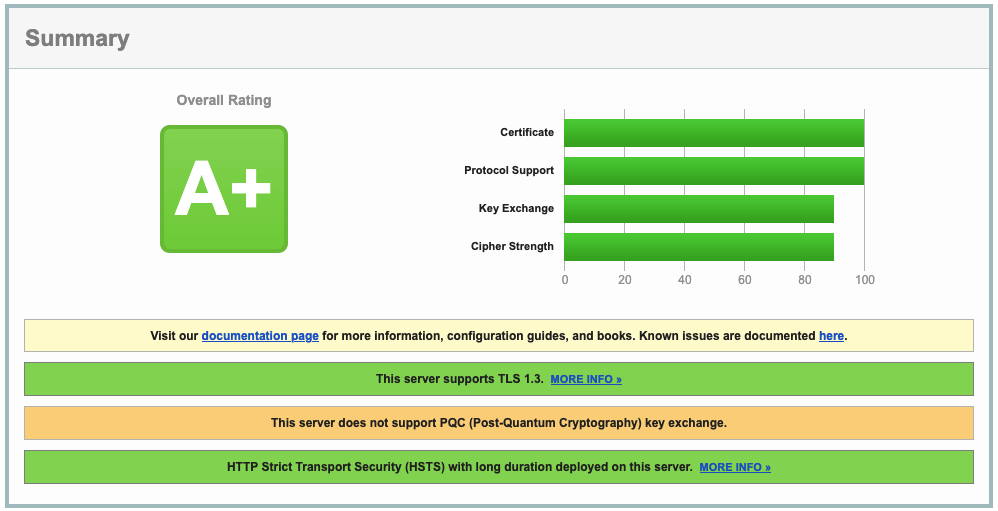
\includegraphics[width=\textwidth]{screenshots/qualys_summary.png}
  \caption{Qualys-Gesamtbewertung: A+.}
  \label{fig:b-summary}
\end{figure}

\textbf{Zertifikat.} Das Server-Zertifikat (Abb.~\ref{fig:b-cert}) ist von Let's Encrypt ausgestellt (Issuer \texttt{R12}, darüber \texttt{ISRG Root X1} als Root). Es verwendet einen RSA-2048-Schlüssel und die Signatur \texttt{SHA256withRSA}, beides aktuell als sicher eingestuft. Der \texttt{Subject Alternative Name} entspricht genau dem Hostnamen \texttt{nwsmooc.mooin.org}, es gibt also keinen Name-Mismatch. Die Laufzeit beträgt ca. 90 Tage (14.\,Mai bis 12.\,Aug. 2026), was typisch für Let's Encrypt ist. Die Chain ist vollständig (zwei Zertifikate, \texttt{Chain issues: None}), das Zertifikat ist in allen großen Trust-Stores (Mozilla, Apple, Android, Java, Windows) als vertrauenswürdig hinterlegt, Certificate Transparency ist erfüllt und der Revocation-Status ist \texttt{Good}.
\begin{figure}[H]
  \centering
  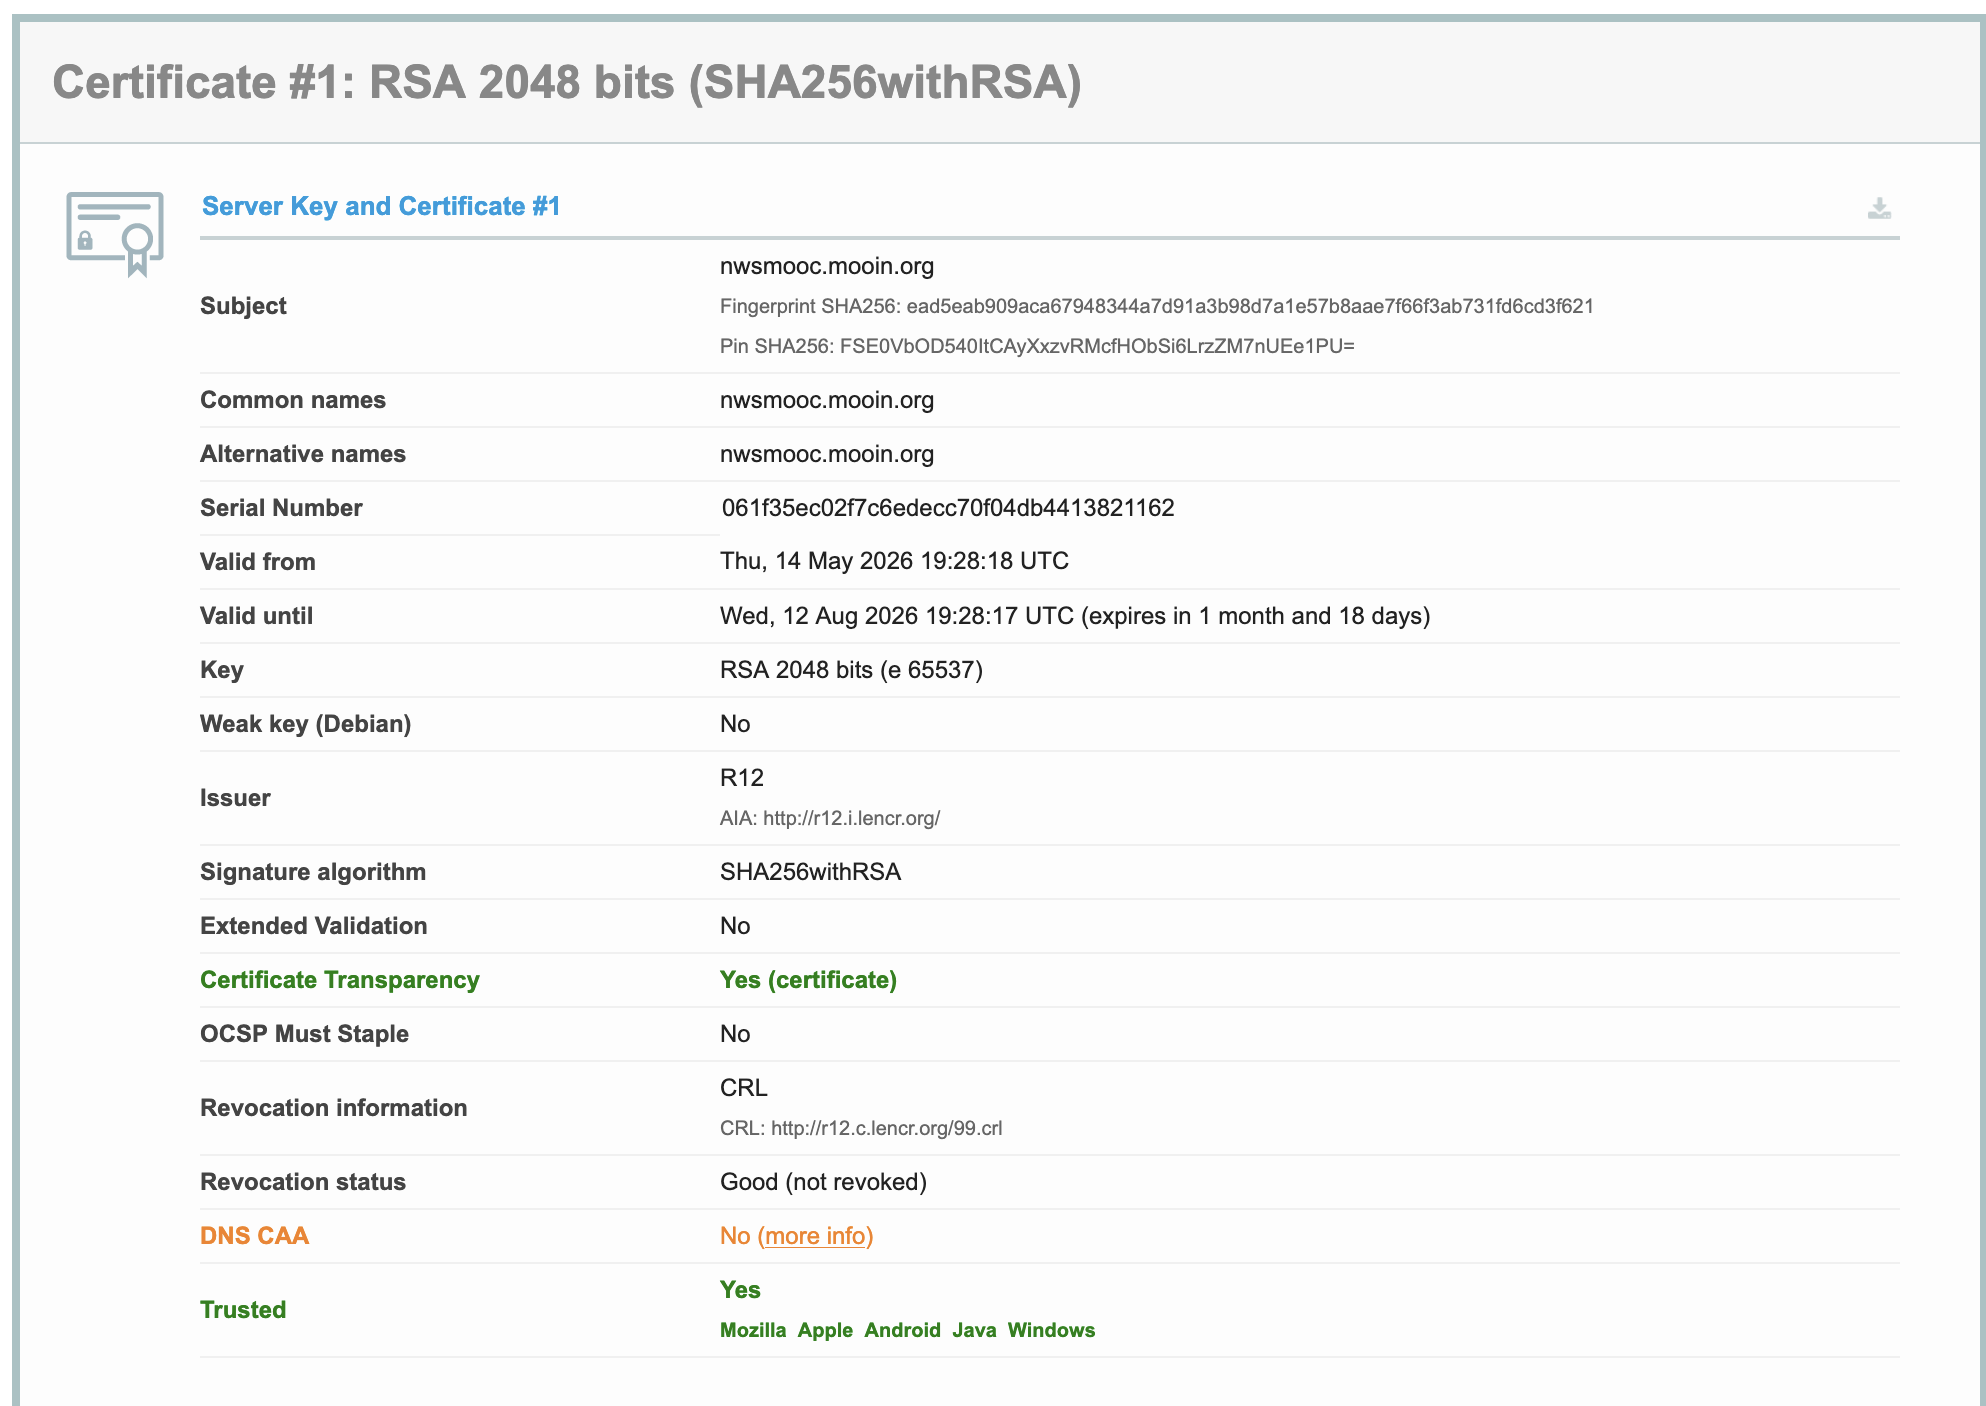
\includegraphics[width=\textwidth]{screenshots/qualys_cert.png}
  \caption{Zertifikatsdetails: Let's Encrypt, RSA 2048, vollständige Chain, allen Stores vertrauenswürdig.}
  \label{fig:b-cert}
\end{figure}

\textbf{Protokolle und Cipher Suites.} Der Server bietet ausschließlich TLS 1.2 und TLS 1.3 an (Abb.~\ref{fig:b-config}). Alle veralteten Protokolle (TLS 1.1, TLS 1.0, SSL 3, SSL 2) sind deaktiviert, was die hohe Protocol-Support-Wertung erklärt. Bei den Cipher Suites werden ausnahmslos Verfahren mit Forward Secrecy (ECDHE bzw. DHE) und AEAD-Verschlüsselung (AES-GCM, ChaCha20-Poly1305) eingesetzt. Veraltete oder bekannt schwache Verfahren wie RC4 oder CBC-basierte Suiten fehlen vollständig.
\begin{figure}[H]
  \centering
  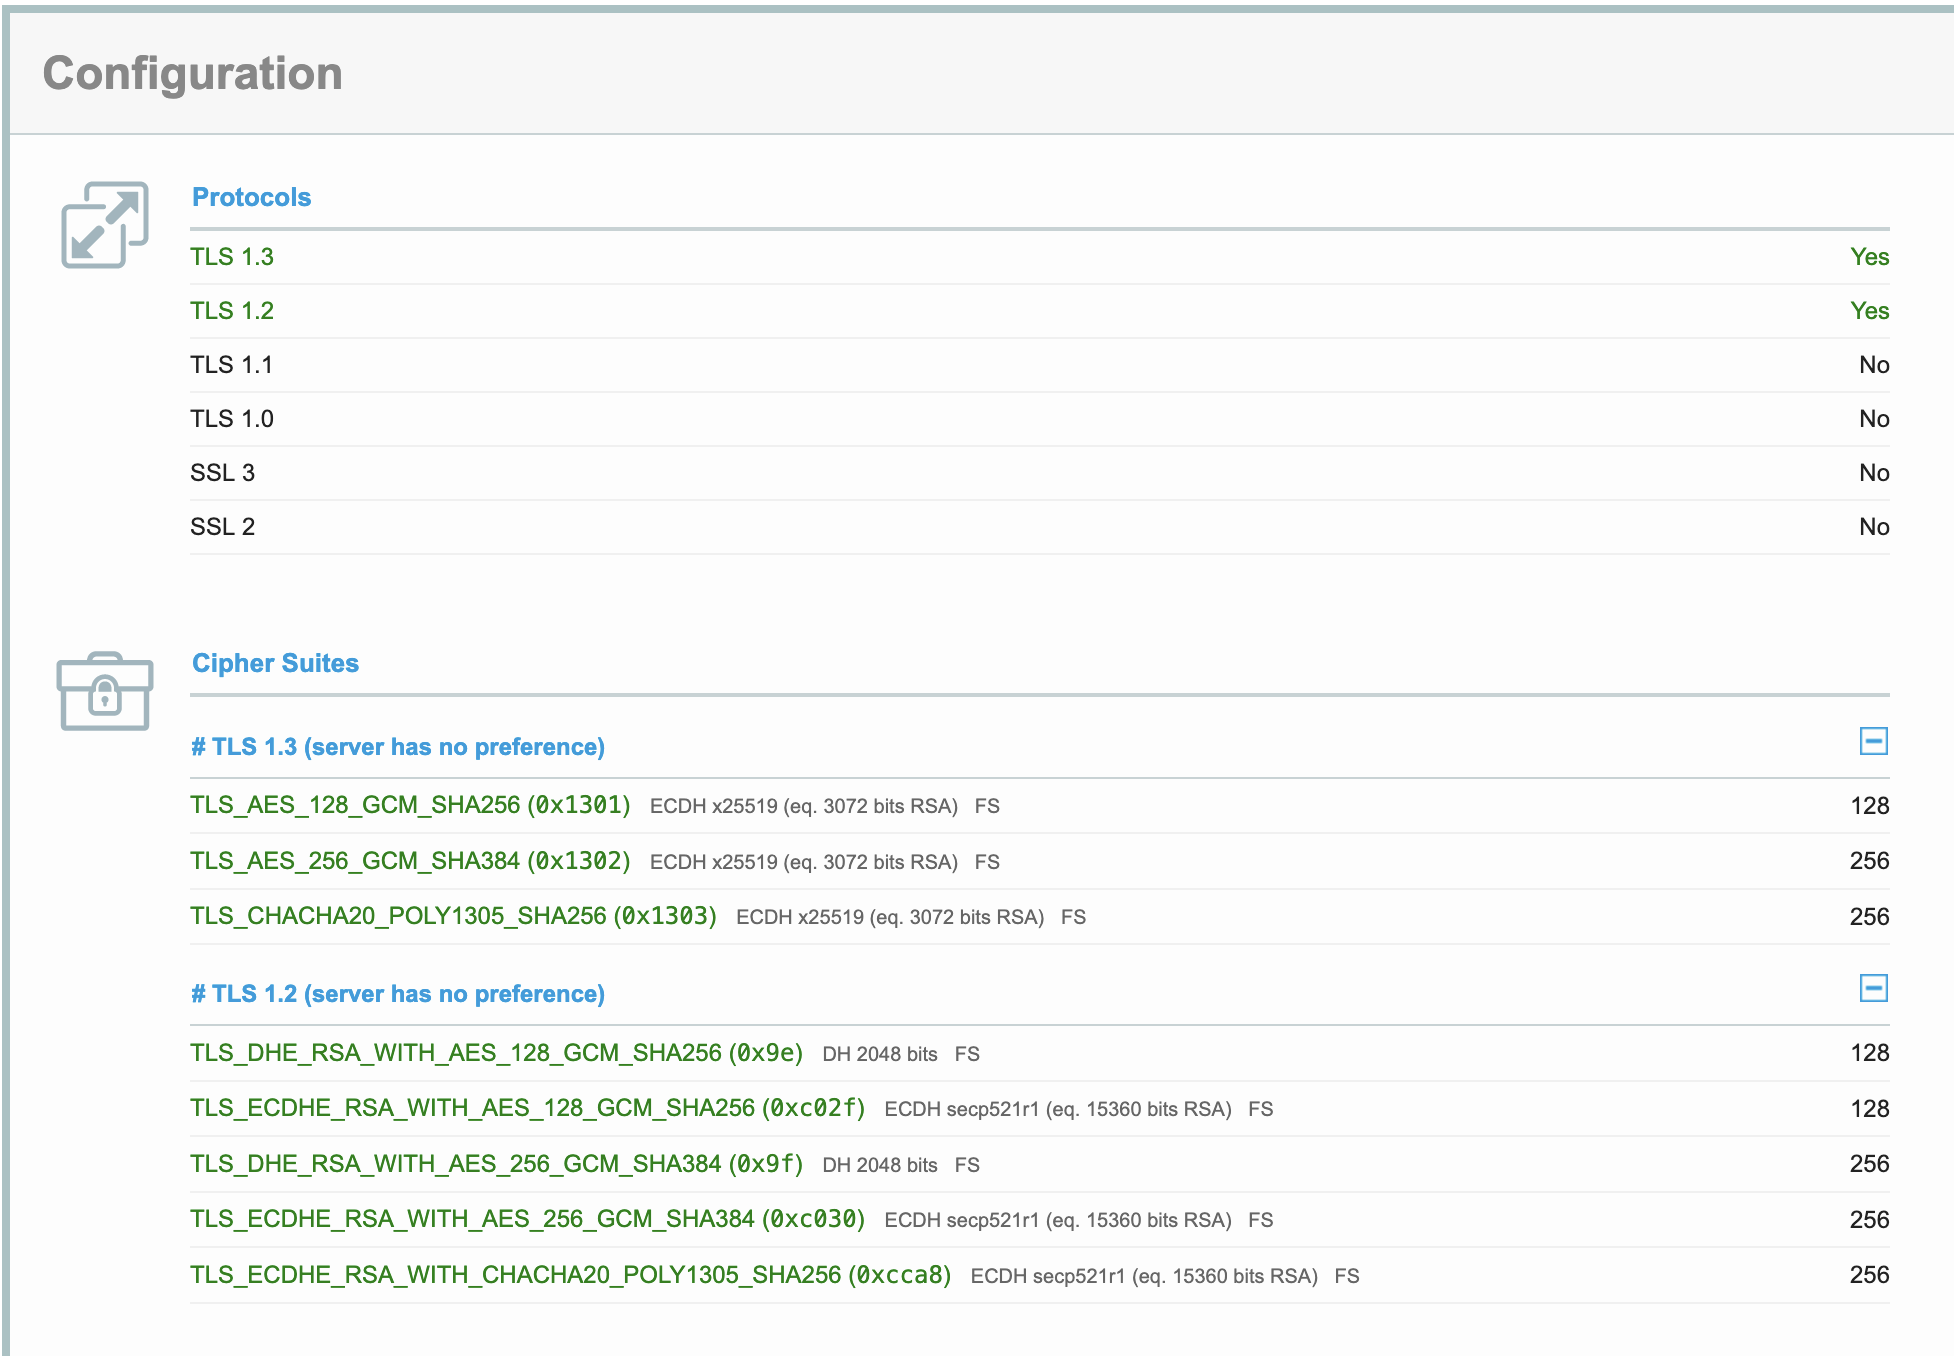
\includegraphics[width=\textwidth]{screenshots/qualys_config.png}
  \caption{Configuration (Ausschnitt): Nur TLS 1.2 und 1.3 aktiv, ausschließlich FS- und AEAD-Cipher-Suites.}
  \label{fig:b-config}
\end{figure}

\textbf{Handshake Simulation.} Die Handshake-Simulation (Abb.~\ref{fig:b-handshake}) prüft, welche TLS-Version und welchen Cipher verschiedene reale Clients aushandeln würden. Aktuelle Browser und Betriebssysteme verbinden sich hiernach problemlos über TLS 1.3 oder TLS 1.2, durchgehend mit Forward Secrecy. Sehr alte Clients (z.\,B. IE 11 auf Windows Phone 8.1 sowie Safari 6/7/8 auf älteren macOS-Versionen) scheitern hingegen mit \texttt{handshake\_failure}.
\begin{figure}[H]
  \centering
  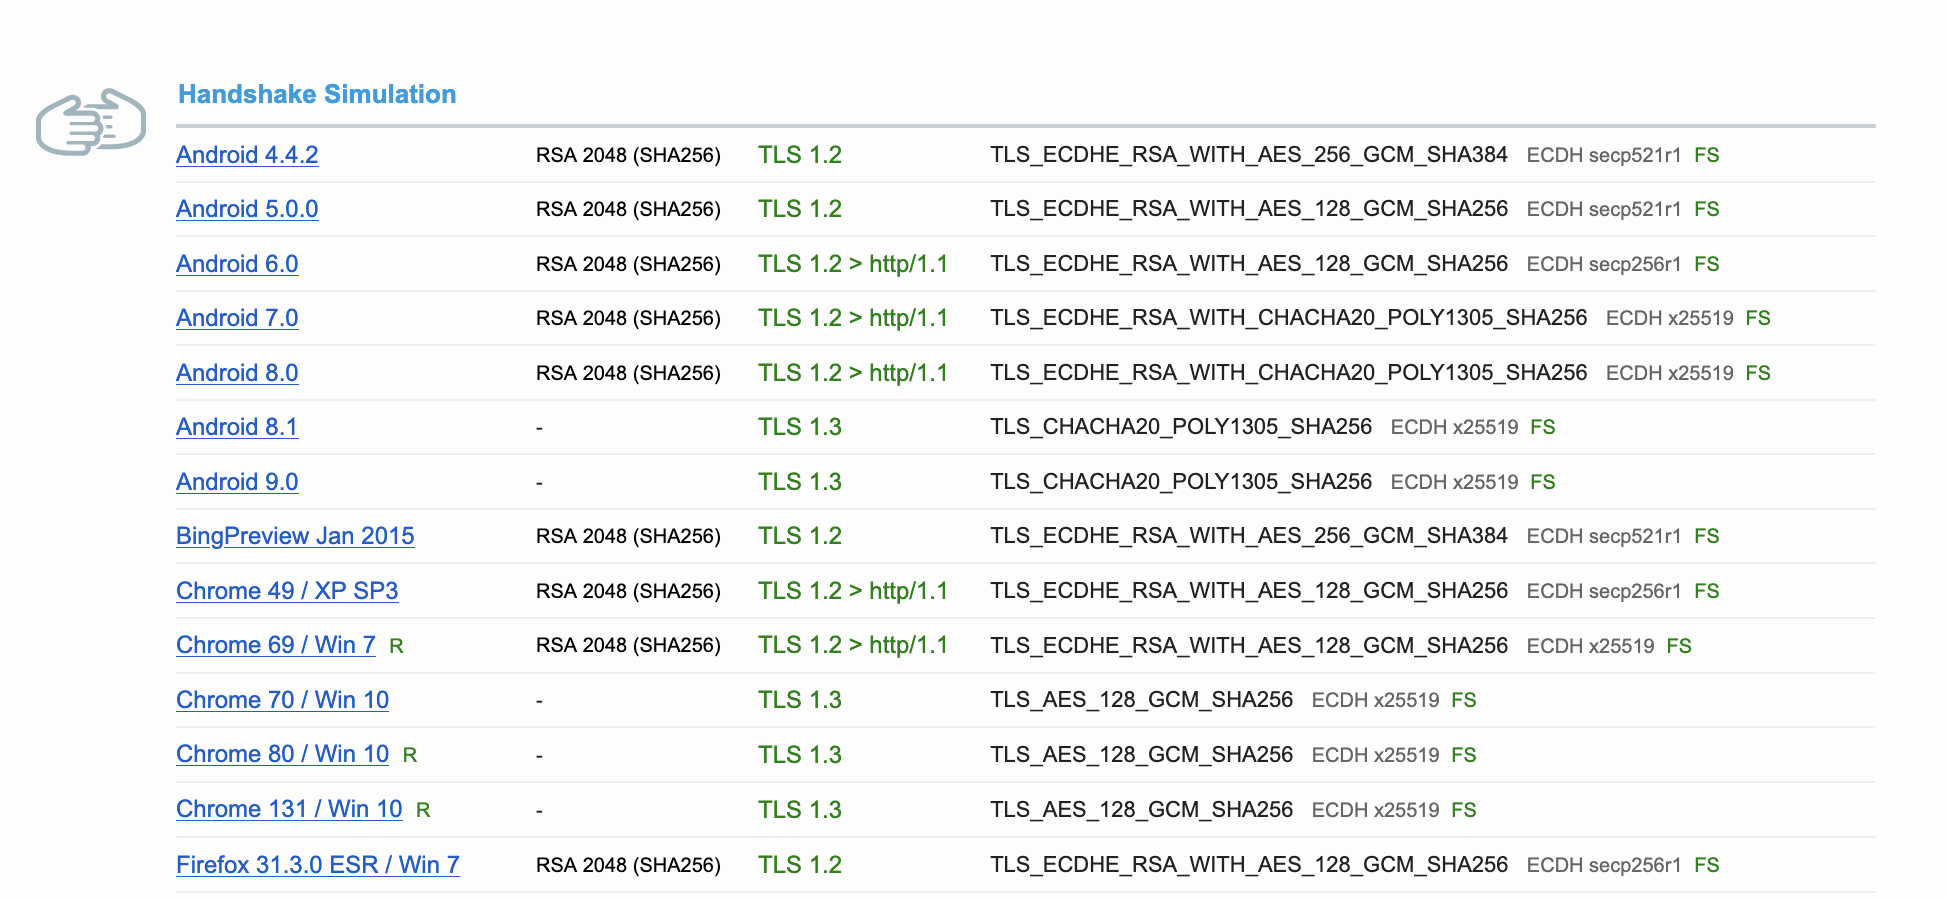
\includegraphics[width=\textwidth]{screenshots/qualys_handshake.png}
  \caption{Handshake-Simulation: moderne Clients mit TLS 1.3/1.2, alte Clients scheitern mit \texttt{handshake\_failure}.}
  \label{fig:b-handshake}
\end{figure}

\textbf{Protocol Details.} Die Detailprüfungen (Abb.~\ref{fig:b-details}) bestätigen das Bild: BEAST ist serverseitig mitigiert, bekannte Angriffe wie POODLE, Heartbleed, RC4 und ROBOT klappen nicht, und ein Downgrade-Schutz über \texttt{TLS\_FALLBACK\_SCSV} ist vorhanden. Forward Secrecy wird als \texttt{ROBUST} eingestuft, HSTS ist mit langer \texttt{max-age}, \texttt{includeSubDomains} und \texttt{preload} gesetzt. Als kleine Schwachpunkte bleiben lediglich fehlendes OCSP Stapling, kein gesetzter DNS-CAA-Eintrag und die noch nicht erfolgte Aufnahme in die HSTS-Preload-Listen der Browser. Keiner dieser Punkte ist kritisch, das Gesamtergebnis bleibt also bei A+.
\begin{figure}[H]
  \centering
  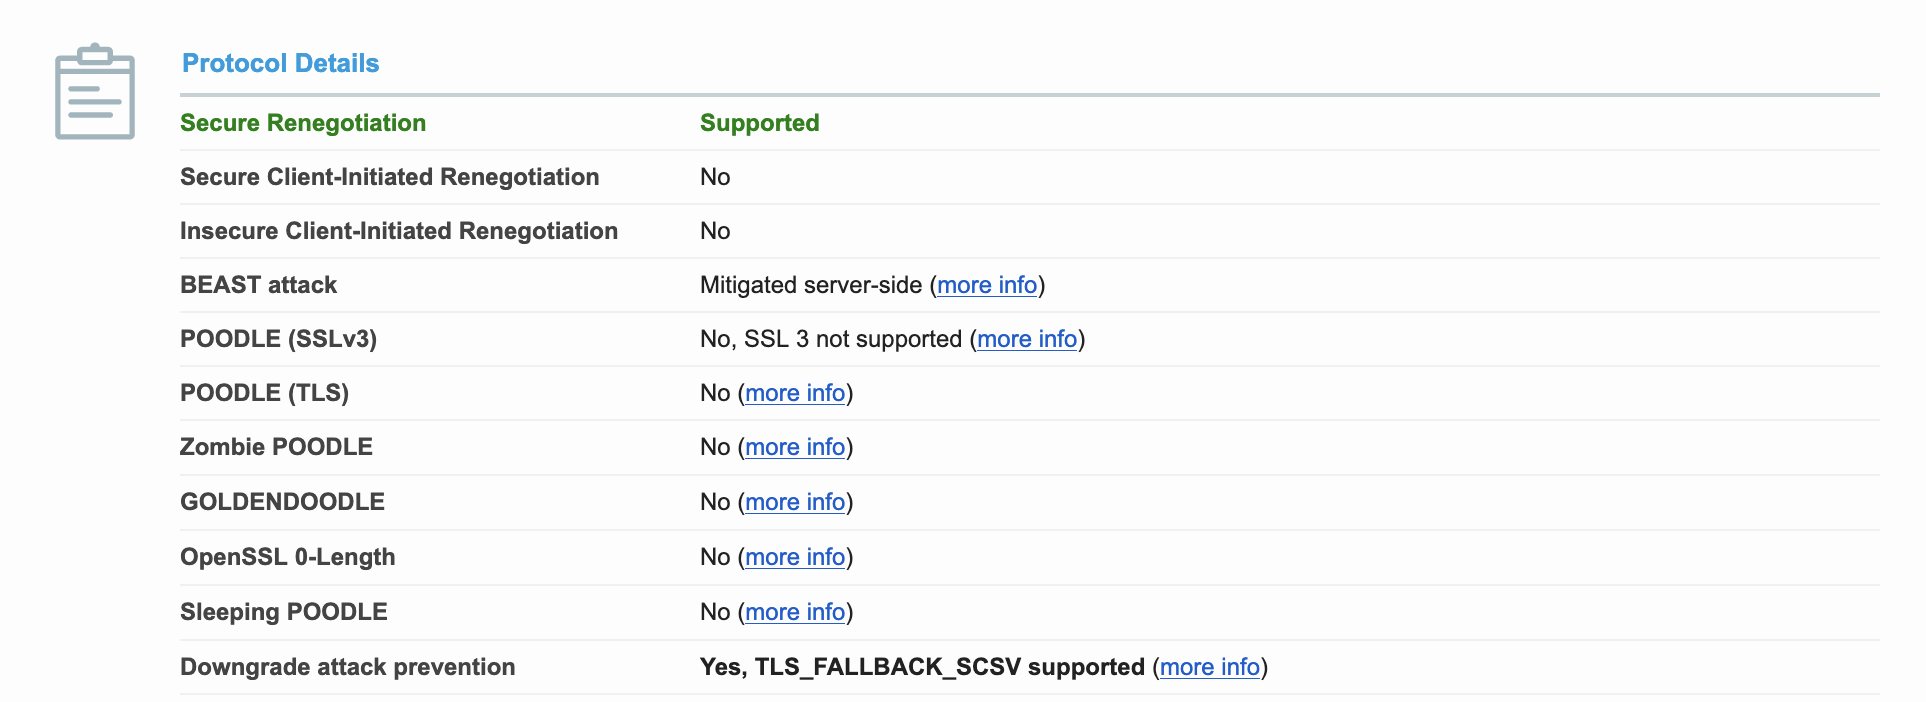
\includegraphics[width=\textwidth]{screenshots/qualys_details.png}
  \caption{Protocol Details (Ausschnitt): gängige Angriffe wirkungslos, Forward Secrecy robust, HSTS aktiv.}
  \label{fig:b-details}
\end{figure}
\subsection{Vergleich: \glqq Recent Worst\grqq{}}
Als Gegenbeispiel aus der \glqq Recent Worst\grqq{}-Liste wurde zufällig \texttt{www.aviation.or.kr} gewählt, das von Qualys mit der schlechtesten Note \textbf{F} bewertet wird (Abb.~\ref{fig:b-worst-summary}). Auffällig ist zunächst, dass das Zertifikat selbst unauffällig ist: Es stammt von GlobalSign, nutzt RSA 2048 mit \texttt{SHA256withRSA}, ist gültig und in allen großen Trust-Stores als vertrauenswürdig hinterlegt (\texttt{Trusted: Yes}). Die F resultiert also nicht aus dem Zertifikat, sondern ausschließlich aus der Konfiguration des Servers.
\begin{figure}[H]
  \centering
  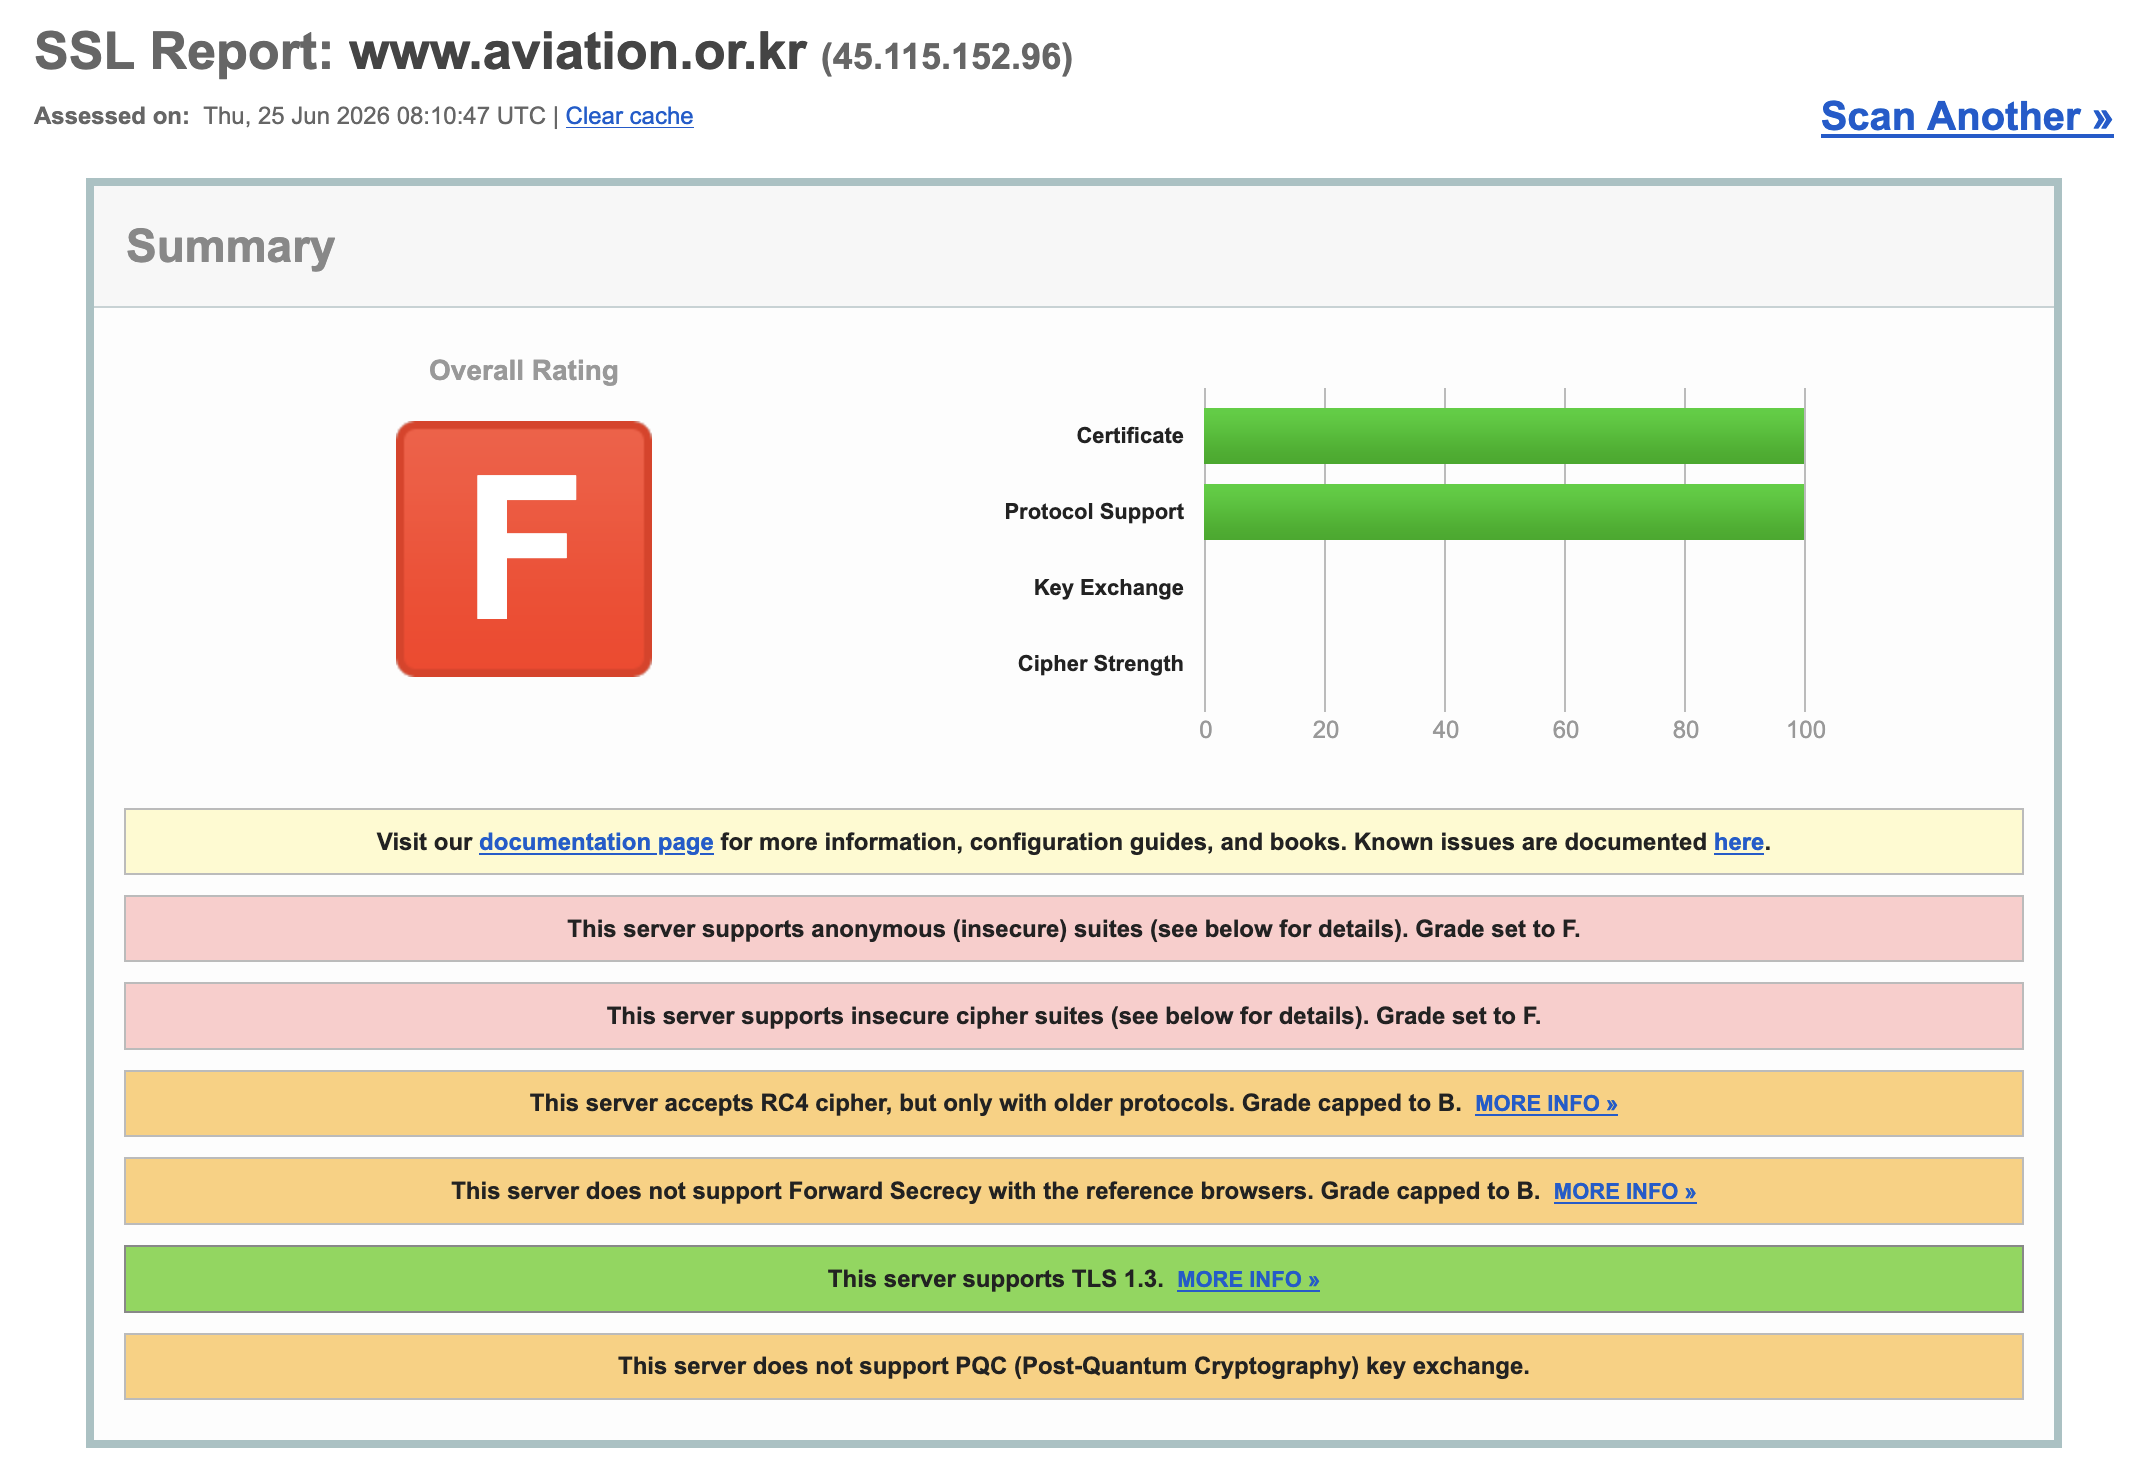
\includegraphics[width=\textwidth]{screenshots/worst_summary.png}
  \caption{\texttt{www.aviation.or.kr}: Summary:Gesamtnote F, Zertifikat dennoch vertrauenswürdig.}
  \label{fig:b-worst-summary}
\end{figure}

Die Summary nennt die Ursachen: Der Server bietet \emph{anonyme} und \emph{unsichere} Cipher Suites an, was jeweils zur Abwertung auf F führt. Zusätzlich akzeptiert er den veralteten RC4-Cipher und unterstützt mit den Referenz-Browsern keine Forward Secrecy. Diese beiden letzten Punkte würden die Note für sich genommen bereits auf B anheben, gehen hier aber in der schwerwiegenderen F unter.

Im Detail der Cipher-Suite-Liste (Abb.~\ref{fig:b-worst-ciphers}) zeigen sich die ausschlaggebenden Verfahren, von Qualys rot als \texttt{INSECURE} markiert:
\begin{itemize}
  \item \textbf{NULL-Ciphers} (z.\,B. \texttt{TLS\_RSA\_WITH\_NULL\_SHA256}): Diese Suiten authentifizieren zwar, verschlüsseln die Nutzdaten aber überhaupt nicht. Die Verbindung wäre damit vollständig im Klartext mitlesbar. Die Cipher-Stärke wird entsprechend mit \texttt{0} angegeben.
  \item \textbf{Anonyme Ciphers} (z.\,B. \texttt{TLS\_ECDH\_anon\_WITH\_NULL\_SHA}): Hier fehlt die Authentifizierung des Servers komplett. Ohne Server-Authentifizierung ist das Zertifikat wirkungslos, da sich ein Angreifer per Man-in-the-Middle dazwischenschalten kann, ohne ein gültiges Zertifikat besitzen zu müssen.
\end{itemize}
Darüber hinaus enthält die Liste zahlreiche als \texttt{WEAK} markierte Suiten (CBC-Verfahren, 1024-Bit-DH, 3DES), die zwar nicht allein für die F verantwortlich sind, aber klar die veraltete, nicht gepflegte Konfiguration darstellen.
\begin{figure}[H]
  \centering
  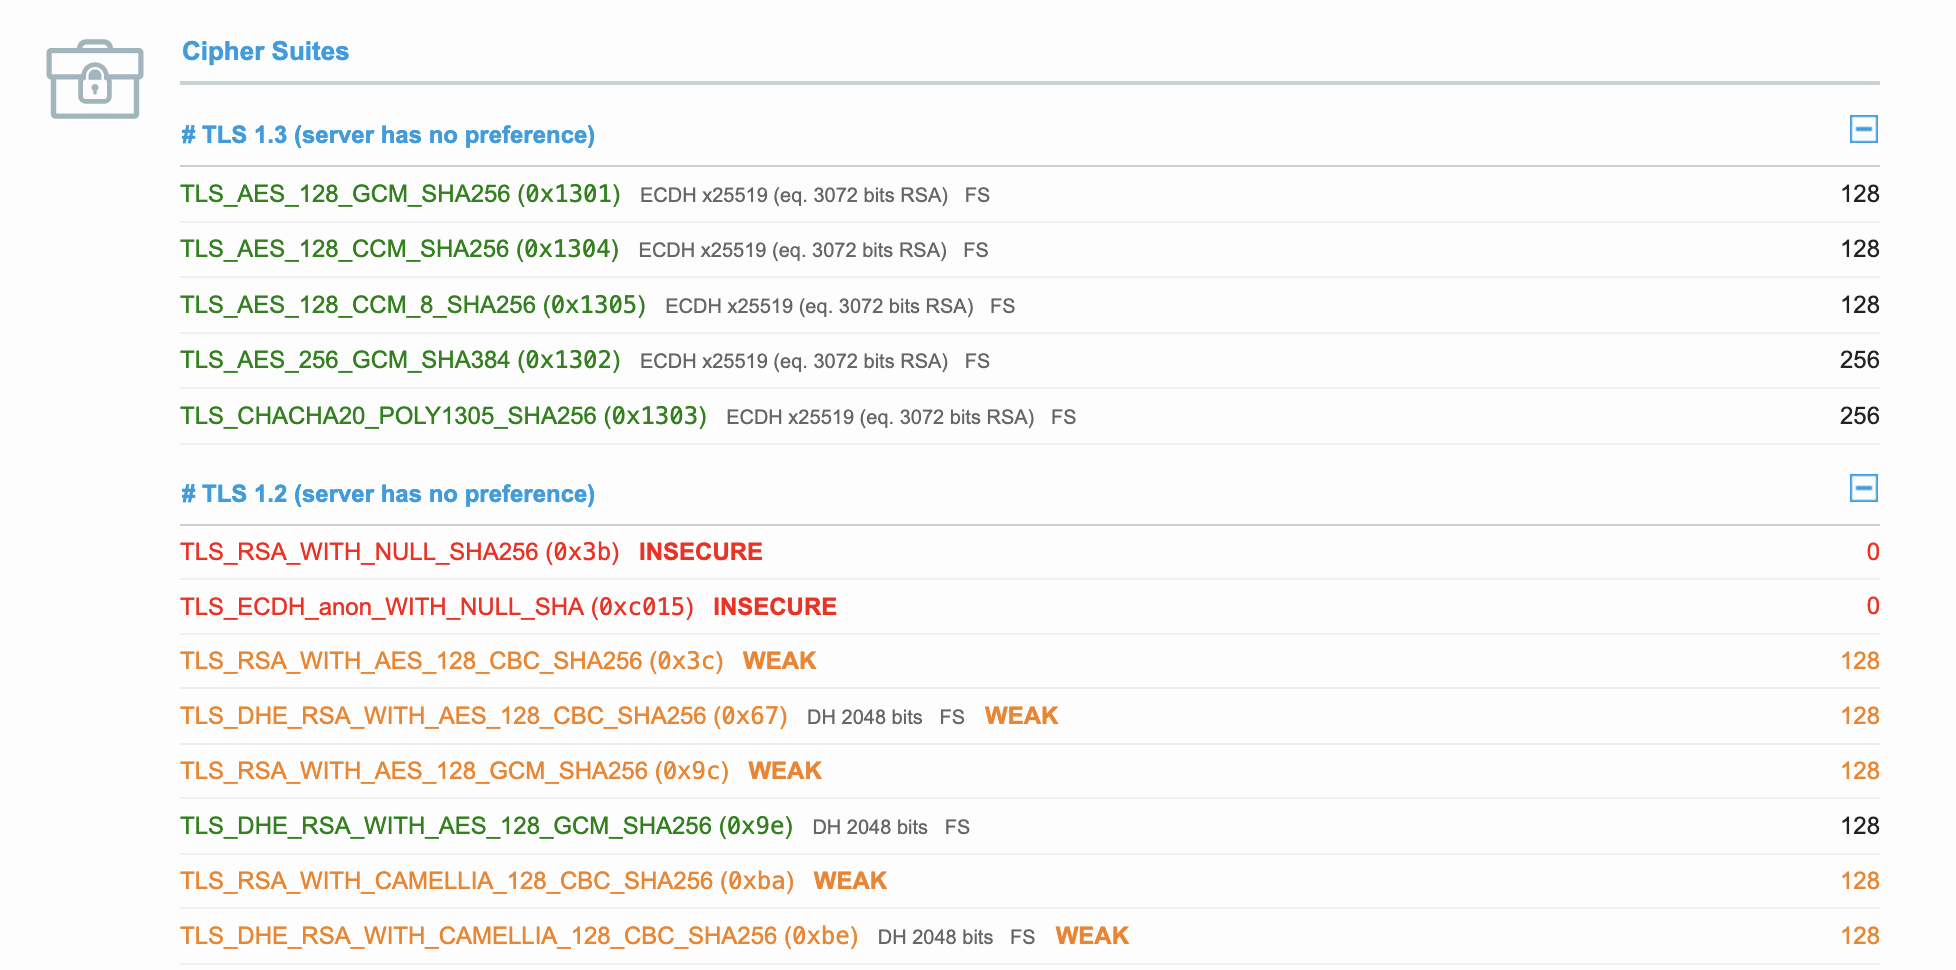
\includegraphics[width=\textwidth]{screenshots/worst_ciphers.png}
  \caption{Cipher Suites (Ausschnitt): Anonyme und NULL-Cipher-Suites (\texttt{INSECURE}, Stärke 0) als Ursache der F-Bewertung.}
  \label{fig:b-worst-ciphers}
\end{figure}

Der Vergleich verdeutlicht den Unterschied zu \texttt{nwsmooc.mooin.org}: Beide Server besitzen ein gültiges, vertrauenswürdiges Zertifikat. Während der Testserver jedoch ausschließlich moderne Protokolle und FS-Cipher-Suites anbietet (A+), schleppt \texttt{www.aviation.or.kr} eine große Menge veralteter und teils völlig unsicherer Verfahren mit. Ein einziges angebotenes NULL- oder anonymes Verfahren genügt bereits, um die gesamte ggf. sonst akzeptable Konfiguration auf die schlechteste Note runter zu ziehen.
% =====================================================================
%  c) Zertifikate im Browser (Firefox & Chrome)
% =====================================================================
\section{Zertifikate im Browser: gültig, abgelaufen, zurückgerufen}
Über die von SSL.com bereitgestellten Beispielzertifikate\footnote{\url{https://www.ssl.com/sample-valid-revoked-and-expired-ssl-tls-certificates/}} soll das Verhalten von Firefox und Chrome bei gültigen, abgelaufenen und zurückgerufenen Zertifikaten direkt verglichen werden. Jedes der drei Zertifikate wurde in beiden Browsern aufgerufen. Verwendet wurde durchgehend das ECC-Set (\texttt{test-dv-ecc}, \texttt{expired-ecc-ev}, \texttt{revoked-ecc-ev}), damit der einzige Unterschied in den Browsern bleibt und nicht zusätzlich beim Zertifikatstyp.

\subsection{Gültiges Zertifikat}
Das gültige Zertifikat (\texttt{test-dv-ecc.ssl.com}) wird in beiden Browsern ohne Beanstandung geladen. Die Kette löst zu einem vertrauenswürdigen Root auf, das Schloss ist geschlossen und die Verbindung wird als sicher ausgewiesen (Abb.~\ref{fig:c-valid}). Firefox nennt zusätzlich den Aussteller (\texttt{SSL Corporation}). Dieser Fall kann als Referenz für das Standardverhalten angesehen werden.
\begin{figure}[H]
  \centering
  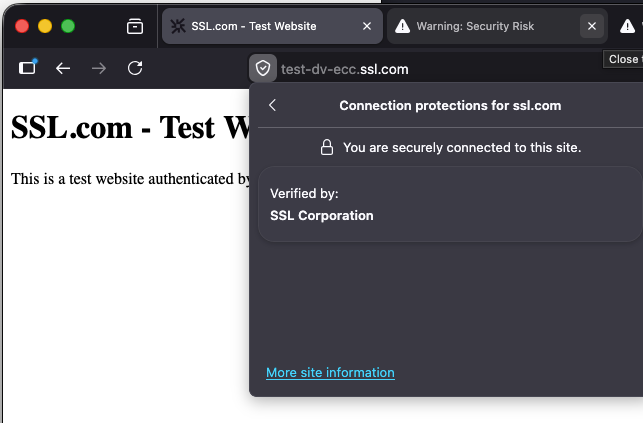
\includegraphics[width=0.7\textwidth]{screenshots/ff-valid.png}
  \caption{Gültiges Zertifikat: Verbindung sicher, Aussteller bestätigt (Firefox). Chrome zeigt identisches Verhalten.}
  \label{fig:c-valid}
\end{figure}

\subsection{Abgelaufenes Zertifikat}
Das abgelaufene Zertifikat (\texttt{expired-ecc-ev.ssl.com}) wird von beiden Browsern mit einer ganzseitigen Warnseite blockiert. Interessant ist, dass beide denselben Sachverhalt mit \emph{unterschiedlichen} Fehlercodes melden:
\begin{itemize}
  \item \textbf{Chrome:} \texttt{NET::ERR\_CERT\_AUTHORITY\_INVALID}
  \item \textbf{Firefox:} \texttt{SEC\_ERROR\_EXPIRED\_CERTIFICATE}
\end{itemize}
Das Zertifikat stammt aus dem Jahr 2019 (ausgestellt am 17.\,Aug. 2019, gültig bis 18.\,Aug. 2019, also nur einen Tag) und wurde von der \texttt{SSL.com EV SSL Intermediate CA ECC R2} signiert (Abb.~\ref{fig:c-expired-cert}). Die beiden Fehlercodes bedeuten Verschiedenes: \texttt{AUTHORITY\_INVALID} heißt, dass keine vertrauenswürdige Kette zum Aussteller gebaut werden kann; \texttt{EXPIRED\_CERTIFICATE} heißt, dass dem Aussteller vertraut wird, aber die Gültigkeit abgelaufen ist.

Der Unterschied erklärt sich über die unterschiedlichen Trust-Stores und die Reihenfolge der Prüfung. Firefox baut über den Mozilla-Trust-Store eine vertrauenswürdige Kette auf, gelangt bis zur Datumsprüfung und meldet also korrekt die abgelaufene Gültigkeit. Die Warnseite benennt das sogar (\glqq Zertifikat abgelaufen am 8/18/2019\grqq{}) und vergleicht mit der Systemzeit (Abb.~\ref{fig:c-expired-ff}). Chrome findet mit dem Chrome Root Store keine vertrauenswürdige Kette zur alten Aussteller-CA und scheitert somit bereit an diesem früheren Schritt, weshalb \texttt{AUTHORITY\_INVALID} gemeldet wird (Abb.~\ref{fig:c-expired-chrome}). Die ebenfalls vorhandene Expiry ist hier nur der zweite, nicht der ausgegebene Fehler. Beide Browser verweigern also korrekt, benennen aber jeweils die Ursache, an der ihre Prüfung zuerst scheitert.
\begin{figure}[H]
  \centering
  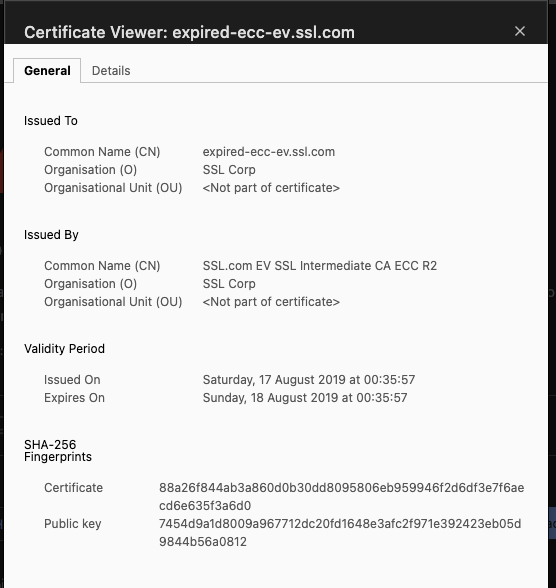
\includegraphics[width=0.6\textwidth]{screenshots/chrome-expired-cert.png}
  \caption{Das abgelaufene Zertifikat: Gültigkeit nur am 17./18.\,Aug. 2019, Aussteller \texttt{SSL.com EV SSL Intermediate CA ECC R2}.}
  \label{fig:c-expired-cert}
\end{figure}
\begin{figure}[H]
  \centering
  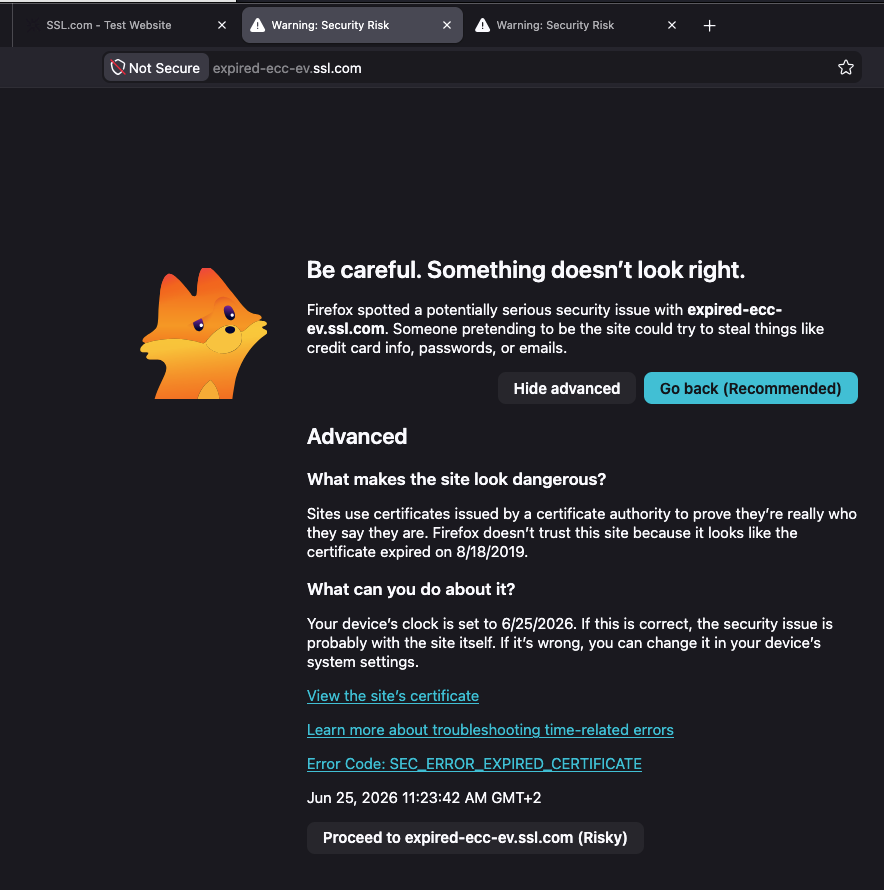
\includegraphics[width=0.8\textwidth]{screenshots/ff-exp.png}
  \caption{Firefox: \texttt{SEC\_ERROR\_EXPIRED\_CERTIFICATE}, mit konkretem Ablaufdatum und Abgleich zur Systemzeit.}
  \label{fig:c-expired-ff}
\end{figure}
\begin{figure}[H]
  \centering
  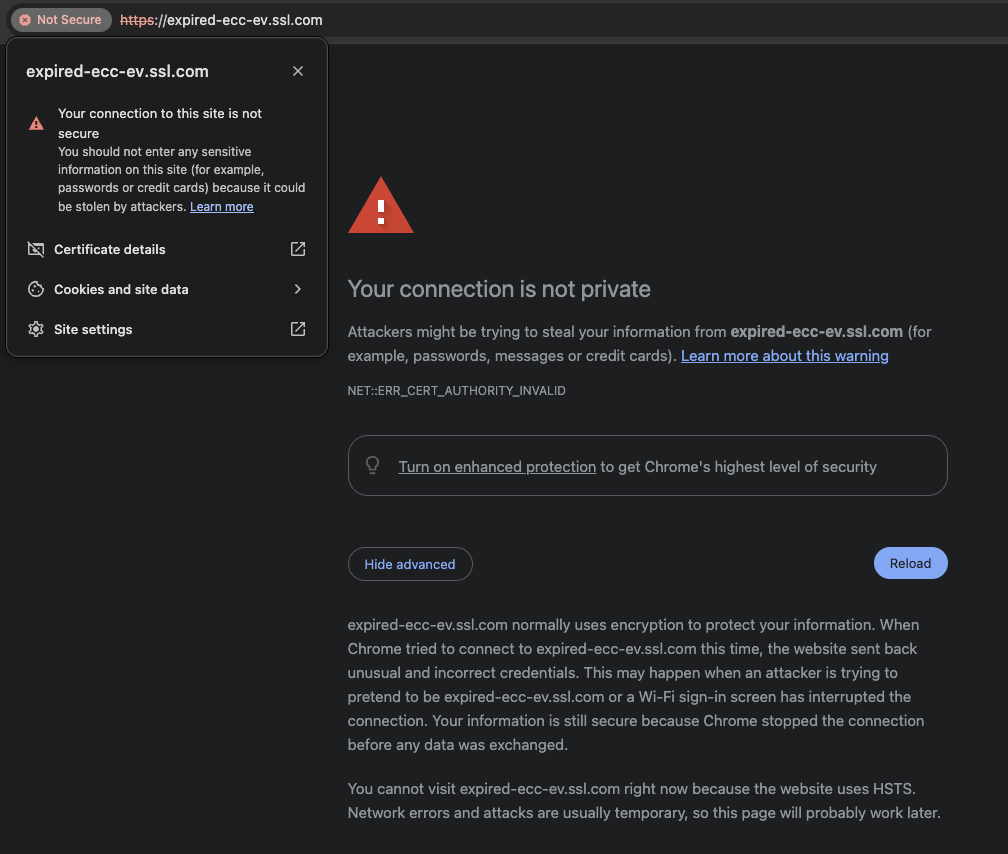
\includegraphics[width=0.8\textwidth]{screenshots/chrome-expired.png}
  \caption{Chrome: \texttt{NET::ERR\_CERT\_AUTHORITY\_INVALID} für dasselbe Zertifikat, da die Kette nicht zu einem vertrauenswürdigen Root auflöst.}
  \label{fig:c-expired-chrome}
\end{figure}

\subsection{Zurückgerufenes (revoked) Zertifikat}
Das zurückgerufene Zertifikat (\texttt{revoked-ecc-ev.ssl.com}) ist der Fall mit dem größten Unterschied, da sich die beiden Browser hier \emph{unterschiedlich} verhalten. Die Gültigkeitsdaten liegen im aktuellen Zeitraum (ausgestellt am 09.\,Juni 2026, gültig bis 24.\,Dez. 2026), das Zertifikat wurde von der CA aber aktiv für ungültig erklärt.
\begin{itemize}
  \item \textbf{Chrome} lädt die Seite ohne Warnung und meldet sogar \glqq Connection is secure\grqq{} und \glqq Certificate is valid\grqq{} (Abb.~\ref{fig:c-revoked-chrome}).
  \item \textbf{Firefox} blockiert mit \texttt{SEC\_ERROR\_REVOKED\_CERTIFICATE} und weist explizit darauf hin, dass das Zertifikat zurückgerufen wurde und nicht mehr vertrauenswürdig ist (Abb.~\ref{fig:c-revoked-ff}).
\end{itemize}
Die Ursache liegt in den unterschiedlichen Sperrprüfungs-Mechanismen. Chrome führt standardmäßig keine Live-OCSP- oder CRL-Abfrage durch, sondern nutzt \emph{CRLSets}, eine von Google selbst gepflegte Liste bekannter Sperrungen. Diese enthält also nur einen Teil aller Widerrufe und ist primär für Notfälle wie kompromittierte CA-Zertifikate gedacht\footnote{\url{https://hacks.mozilla.org/2025/08/crlite-fast-private-and-comprehensive-certificate-revocation-checking-in-firefox/}}. Ein gewöhnliches widerrufenes Endzertifikat wie dieses Testzertifikat ist dort nicht enthalten und wird daher als gültig behandelt. Firefox nutzt seit Version~137 \emph{CRLite}, eine kompakt kodierte, \emph{vollständige} Sperrliste aus den Certificate-Transparency-Logs, die lokal vorgehalten und alle zwölf Stunden aktualisiert wird. Da dieses Zertifikat in den CT-Logs als widerrufen geführt wird, erkennt Firefox den Widerruf zuverlässig und blockiert.

Sicherheitstechnisch ist das das relevanteste Ergebnis dieser Teilaufgabe: Das selbe, von der CA explizit widerrufene, Zertifikat wird vom einen Browser akzeptiert und vom anderen blockiert. Die Wirksamkeit der Sperrprüfung hängt also nicht am Zertifikat, sondern an der Implementierung des Browsers. Ergänzend bleiben serverseitige Maßnahmen wirksam, etwa kurze Zertifikatslaufzeiten zur Begrenzung des Zeitfensters (wie bei Let's Encrypt in Teilaufgabe b) sowie OCSP Stapling bzw. OCSP Must-Staple.
\begin{figure}[H]
  \centering
  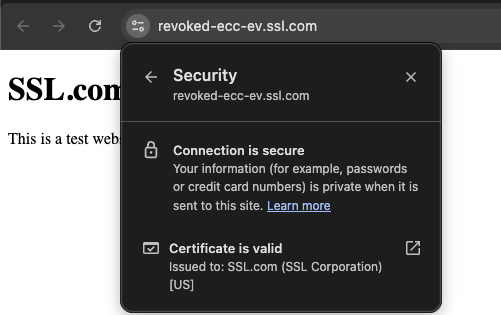
\includegraphics[width=0.7\textwidth]{screenshots/chrome-revoked.png}
  \caption{Chrome akzeptiert das widerrufene Zertifikat: \glqq Certificate is valid\grqq{}, da die Sperrung nicht in den CRLSets enthalten ist.}
  \label{fig:c-revoked-chrome}
\end{figure}
\begin{figure}[H]
  \centering
  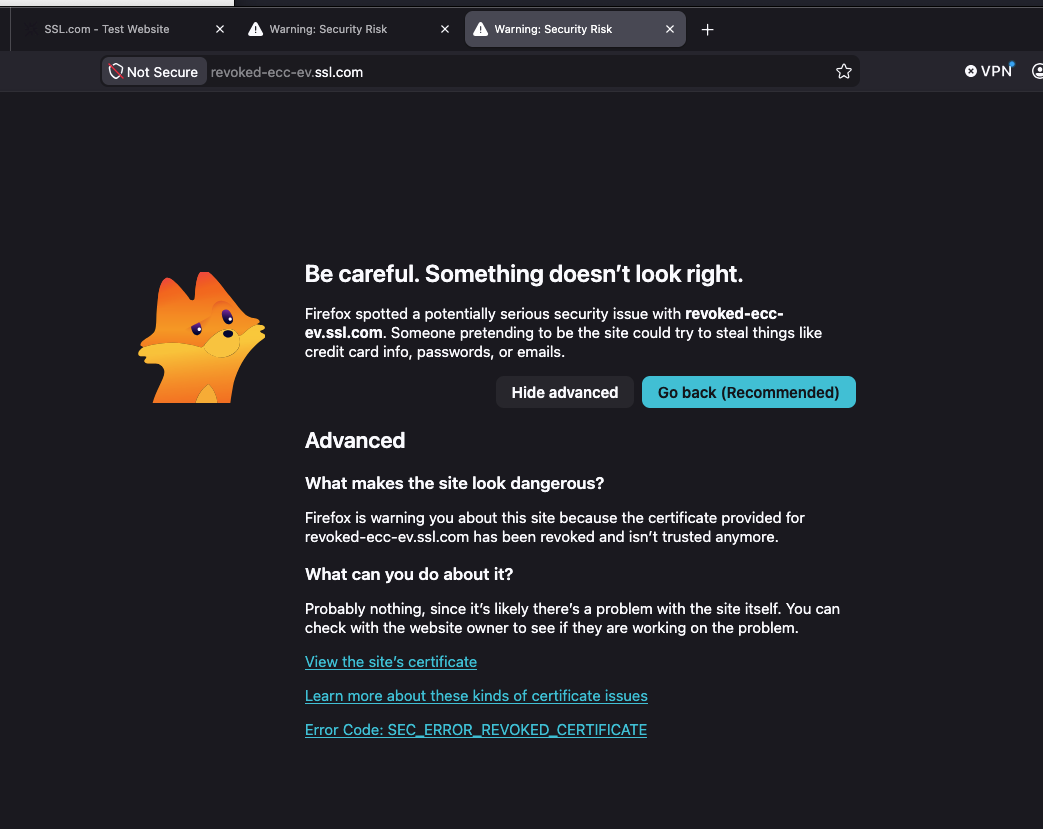
\includegraphics[width=0.8\textwidth]{screenshots/ff-rev.png}
  \caption{Firefox blockiert dasselbe Zertifikat mit \texttt{SEC\_ERROR\_REVOKED\_CERTIFICATE}, da CRLite den Widerruf aus den CT-Logs kennt.}
  \label{fig:c-revoked-ff}
\end{figure}

\subsection{Fazit: Umgang der Browser im Vergleich}
Der Vergleich lässt sich kompakt zusammenfassen:
\begin{table}[H]
  \centering
  \small
  \begin{tabular}{lll}
    \textbf{Zertifikat} & \textbf{Chrome} & \textbf{Firefox} \\
    \hline
    gültig     & geladen, sicher                         & geladen, sicher \\
    abgelaufen & blockiert (\texttt{AUTHORITY\_INVALID}) & blockiert (\texttt{EXPIRED\_CERTIFICATE}) \\
    revoked    & geladen, keine Warnung                  & blockiert (\texttt{REVOKED\_CERTIFICATE}) \\
  \end{tabular}
  \caption{Browser-Verhalten bei den drei Zertifikatstypen.}
  \label{tab:c-vergleich}
\end{table}

Daraus ergibt sich folgendes Fazit: Erstens wird ein \textbf{abgelaufenes} Zertifikat zuverlässig von beiden Browsern erkannt, da dies eine rein lokale Prüfung ist (Abgleich der Gültigkeitsdaten mit der Systemzeit, ohne Netzwerkabfrage). Dass dabei unterschiedliche Fehlercodes erscheinen, zeigt, dass die Bewertung browserspezifisch ist und von Trust-Store und Prüfreihenfolge abhängt, nicht allein vom Zertifikat. Zweitens fällt die Prüfung eines \textbf{zurückgerufenen} Zertifikats je nach Browser unterschiedlich aus: Firefox erkennt den Widerruf dank der vollständigen CRLite-Liste, Chrome hingegen nicht, da seine CRLSets nur einen kleinen Ausschnitt aller Sperrungen abdecken. Auf die Sperrprüfung des Browsers allein ist also nicht wirklich Verlass, für wirksamen Schutz wird das Zusammenspiel von kurzen Laufzeiten und serverseitigem OCSP Stapling benötigt.

% =====================================================================
%  d) SilentEye / Steganographie
% =====================================================================
\section{SilentEye: versteckte, AES256-verschlüsselte Inhalte}
Beide Beispieldateien wurden mit SilentEye dekodiert. In den folgenden Abbildunge nsind die Ergebnisse zu sehen:

\subsection{\texttt{SilentEyeJPGBeispiel.jpg}}
Versteckt an der Header-Position \texttt{bottom}: der Klartext \glqq Verschlüsselte Nachricht in jpg-Bild\grqq{} (Abb.~\ref{fig:d-jpg}).
\begin{figure}[H]
  \centering
  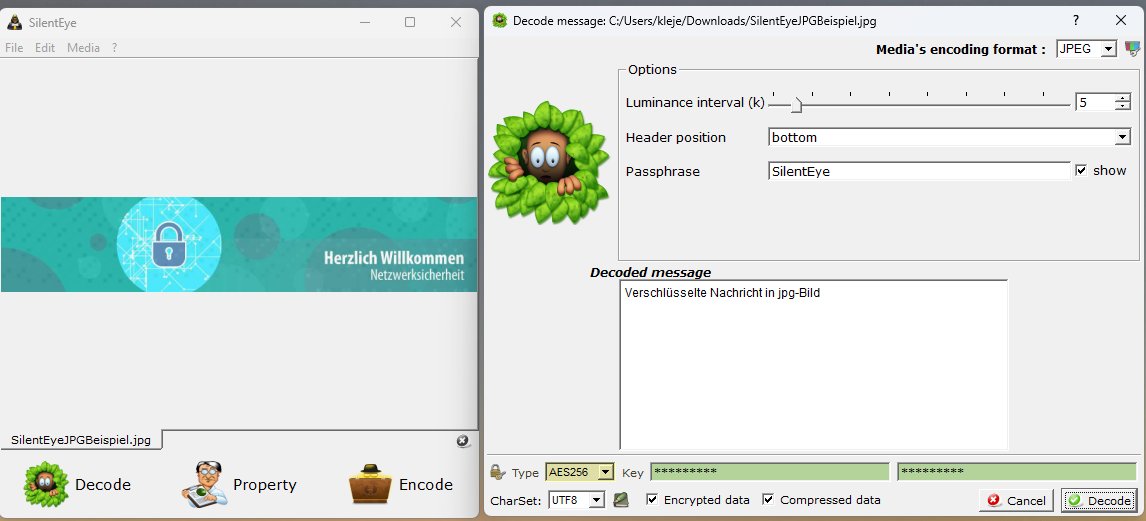
\includegraphics[width=\textwidth]{screenshots/silenteye-jpg-bot.png}
  \caption{JPG-Dekodierung: entschlüsselte Textnachricht.}
  \label{fig:d-jpg}
\end{figure}

\subsection{\texttt{SilentEyeBMPBeispiel.bmp}}
Versteckt an der Header-Position \texttt{signature}: die eingebettete Datei \texttt{bgpszenario.png} (Abb.~\ref{fig:d-bmp}), ein Netzwerktopologie-Diagramm (Abb.~\ref{fig:d-bmp-png}).
\begin{figure}[H]
  \centering
  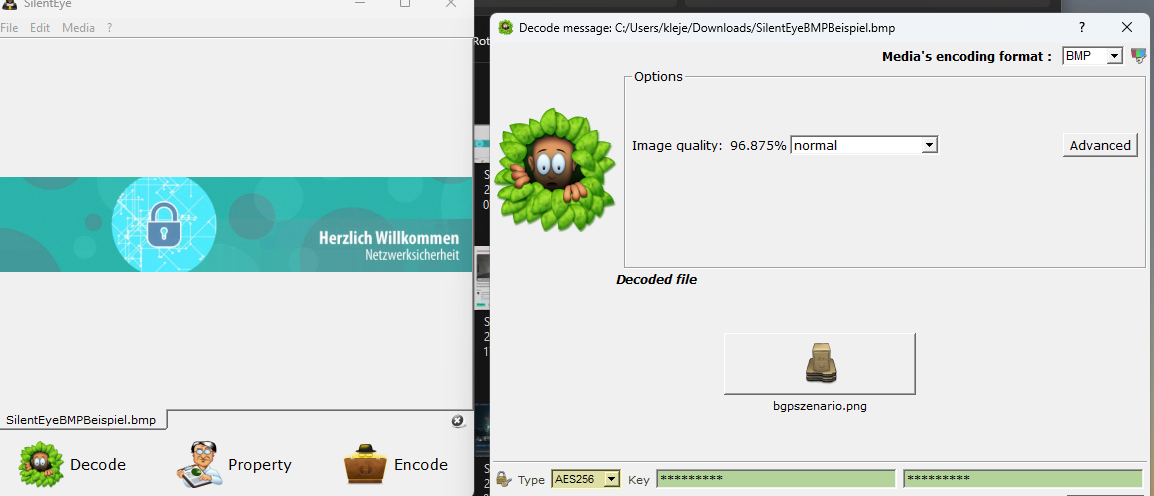
\includegraphics[width=\textwidth]{screenshots/silenteye-bmp.png}
  \caption{BMP-Dekodierung: extrahierte Datei \texttt{bgpszenario.png}.}
  \label{fig:d-bmp}
\end{figure}
\begin{figure}[H]
  \centering
  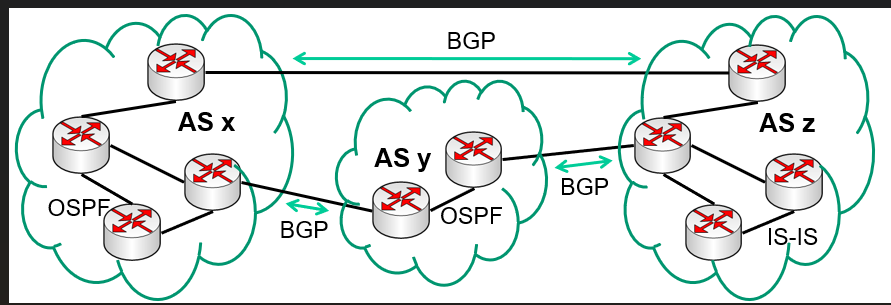
\includegraphics[width=0.8\textwidth]{screenshots/silenteye-bmp-res.png}
  \caption{Inhalt der extrahierten \texttt{bgpszenario.png}.}
  \label{fig:d-bmp-png}
\end{figure}

\end{document}
